\section{Inference}
\label{sec:inference}

Given a labelled network $(A, X)$, we wish to infer if and how the observed features $X$ impact the graphical structure $A$. Formally,
this means characterising the posterior distribution for $\theta$,
$
p(\theta|A, X) \propto p(\theta) \cdot p(A | X, \theta).
$
Therefore, following standard Bayesian practice,
we aim to draw samples from this posterior,
$
	\label{eqn:theta-target}
	\theta^{(t)} \sim p(\theta | A, X).
$
We propose an iterative Markov chain Monte Carlo
(MCMC) approach to obtain these samples
$\{\theta^{(t)}\}$. We first draw a sample $b^{(t)}$ 
from the block membership posterior,
and then use $b^{(t)}$ to obtain a corresponding
sample $\theta^{(t)}$:
%
\begin{equation}
	b^{(t)} \stackrel{\rm distr}{\approx} p \big( b | A, X \big) 
	\quad \textrm{then} \quad
	\theta^{(t)} \stackrel{\rm distr}{\approx} 
	p\big(\theta | X, b^{(t)} \big),
\end{equation}
%
where these approximations become exact as
the number of MCMC iterations $t\to\infty$.
Splitting the Markov chain into two levels side-steps the intractable summation over
all latent $b \in [B]^N$ required to directly compute the likelihood, $p(A| X, \theta)$.
The resulting $\theta^{(t)}$ samples are asymptotically
unbiased in that the expectation of 
their distribution converges to the true posterior.
%
\begin{figure}[!ht]
	\centering
%   IWSM Template does not support tikz
%	\begin{tikzpicture}[
%		scale=0.8, every node/.style={transform shape},
%		roundnode/.style={circle, draw=black, minimum size=12mm},
%		squarednode/.style={rectangle, draw=black, minimum size=12mm}
%		]
%		% nodes
%		\node[roundnode] (b0) at (0, 2) {$b^{(t)}$};
%		\node[roundnode] (b1) at (5, 2) {$b'$};
%		\node[roundnode] (b2) at (10, 2) {$b^{(t+1)}$};
%		\node[roundnode] (t0) at (0, 0) {$\theta^{(t)}$};
%		\node[roundnode] (t1) at (5, 0) {$\theta'$};
%		\node[roundnode] (t2) at (10, 0) {$\theta^{(t+1)}$};
%		
%		% arrows
%		\draw[->] (b0) to node[above] {$\sim q_b ( b^{(t)}, b' | A )$} (b1);
%		\draw[->] (b1) to node[above] {$\alpha_b (b, b' | A )$} (b2);
%		\draw[->] (b0) [out=25, in=155] to node[above] {$1-\alpha_b$} (b2);
%		
%		\draw[->] (t0) to node[above] {$\sim q_\theta(\theta^{(t)}, \theta' | X, b^{(t)})$} (t1);
%		\draw[->] (t1) to node[above] {$\alpha_\theta (\theta, \theta' | X, b^{(t)})$} (t2);
%		\draw[->] (t0) [out=-25, in=-155] to node[below] {$1-\alpha_\theta$} (t2);
%		
%		\draw[dashed, ->] (b0) to (2, 0.8);
%		\draw[dashed, ->] (b0) to (6.5, 0.8);
%		
%	\end{tikzpicture}
	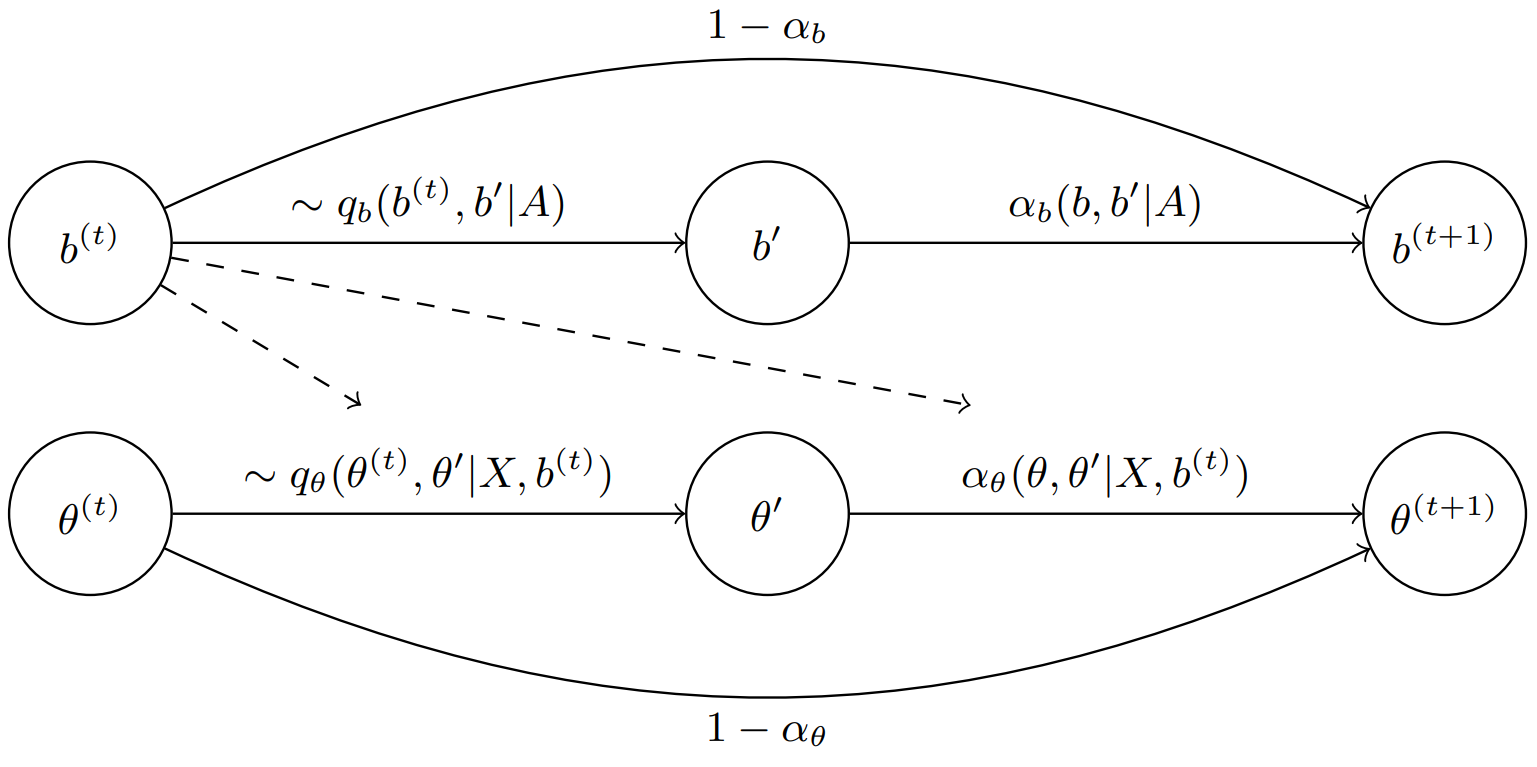
\includegraphics[width=0.6\textwidth]{img/sampling-sequence}
	\caption{$\theta$-sample generation.}
	\label{fig:samp-sequence}
\end{figure}
 
Figure \ref{fig:samp-sequence} shows an overview of the proposed method, with $q$ and $\alpha$ denoting the Metropolis-Hastings proposal distribution and acceptance probability.
Due to the formulation of the FFBM, evaluating $p(b| X)$ does not depend on $X$ so
we do not need $X$ to sample $b$.
And on the other level, in order to obtain 
samples for $\theta$
we use only $b$ but not $A$, as $(\theta \perp \!\!\! \perp A )| b$. 
